\subsection{Anforderungsanalyse mittels Use-Case-Betrachtung}
% TODO: Struktur der Überschriften ändern, diese hat nur einen 
% Unterpunkt und passt thematisch nicht

\subsubsection{Interaktion über Slack}

Es werden folgende Befehle für die Interaktion definiert.

\begin{table}[H]
\centering
\begin{tabular}{l|l}
  Befehl & Bedeutung \\
 \hline
% für vergessliche Leute
 zeige Schicht & zeigt die nächste Schicht für die aufrufende Person an \\
 zeige Schichten & zeigt alle zukünftigen Schichten für die aufrufende Person an \\
 zeige alle Schichten & zeigt einen Schichtplan an, welcher alle Mitglieder enthält \\
 
% jedes Mitglied muss pro Jahr mindestens x mal an die Bar
 zeige Anzahl Schichten & zeigt die geleisteten Schichten für dieses Jahr an \\
 zeige Anzahl alte Schichten & zeigt die geleisteten Sichten für letztes Jahr an \\
 
% zum Anzeigen der Auswahl an welchen man teilnehmen  möchte
 zeige Termine & zeigt alle kommenden Termine $t_i$ an \\
 zeige Veranstaltungen & zeigt alle zukünftigen Veranstaltungen $v_i$ an ($V \subseteq T$) \\
 zeige Sitzungen & zeigt alle zukünftigen Sitzungen $s_i$ an ($S \subseteq T$) \\
 
% für Termin eintragen
 nehme Teil an $t_i$ & trägt den aufrufenden Nutzer als Teilnehmer für $t_i$ ein \\
 nehme nicht Teil an $t_i$ & trägt den aufrufenden Nutzer für $t_i$ aus\\

 % Utilities
 hilf mir & zeigt alle verfügbaren Kommandos an \\
 Danke & bricht die aktuelle Konversation ab
 
 wann ist der nächste termin?
 trag mich ein
 
 
\end{tabular}
\caption{Befehle zur Chatbotinteraktion}
\label{tab:chatbotinteraktion}
\end{table}

Die Befehle in \autoref{tab:chatbotinteraktion} folgen einem vereinfachtem Schema natürlicher Sprache: $<Prädikat (Imperativ)> <Subjekt>$. Die Struktur der Befehle soll dabei einfach zu merken, auf menschlicher Sprache basierend und auch auf mobilen Geräten mit wenig Tipparbeit verwendbar sein. Bei einem optionalen Einsatz einer Spracherkennung sind auch komplexere Satzkonstruktionen möglich, für den hier zu erfüllenden Zweck genügt das Schema aus $<Befehl> <Objekt> <Filter>$. Wie in \cite{ZueConversationalinterfacesadvances2000} beschrieben, weicht die Art der Kommunikation von Mensch-zu-Mensch und Mensch-zu-Bot voneinander ab, worauf bei der Definition der Interaktionsbefehle geachtet wurde. Es ist nach Ansicht der Autoren wenig sinnvoll, einen Bot zu entwickeln, der durch den Zugriff auf große Datenmengen den Eindruck von Intelligenz vermittelt, die aber durch ihre Begrenzung dem Nutzer keinen Mehrwert bietet. Der hier entwickelte Bot verfügt bewusst über ein begrenztes Vokabular, so dass er nur die vom Nutzer gewünschten Informationen liefert; die Kenntnis der Befehle obliegt dem Nutzer.

Aus den in \autoref{tab:chatbotinteraktion} definierten Befehlen wurden die Aktivitätsdiagramme \autoref{img:activity-zeige} und \autoref{img:activity-teilnahme} erstellt, um die Reihenfolge der Interaktion besser zu strukturieren.

\begin{figure}[htbp]
    \centering
    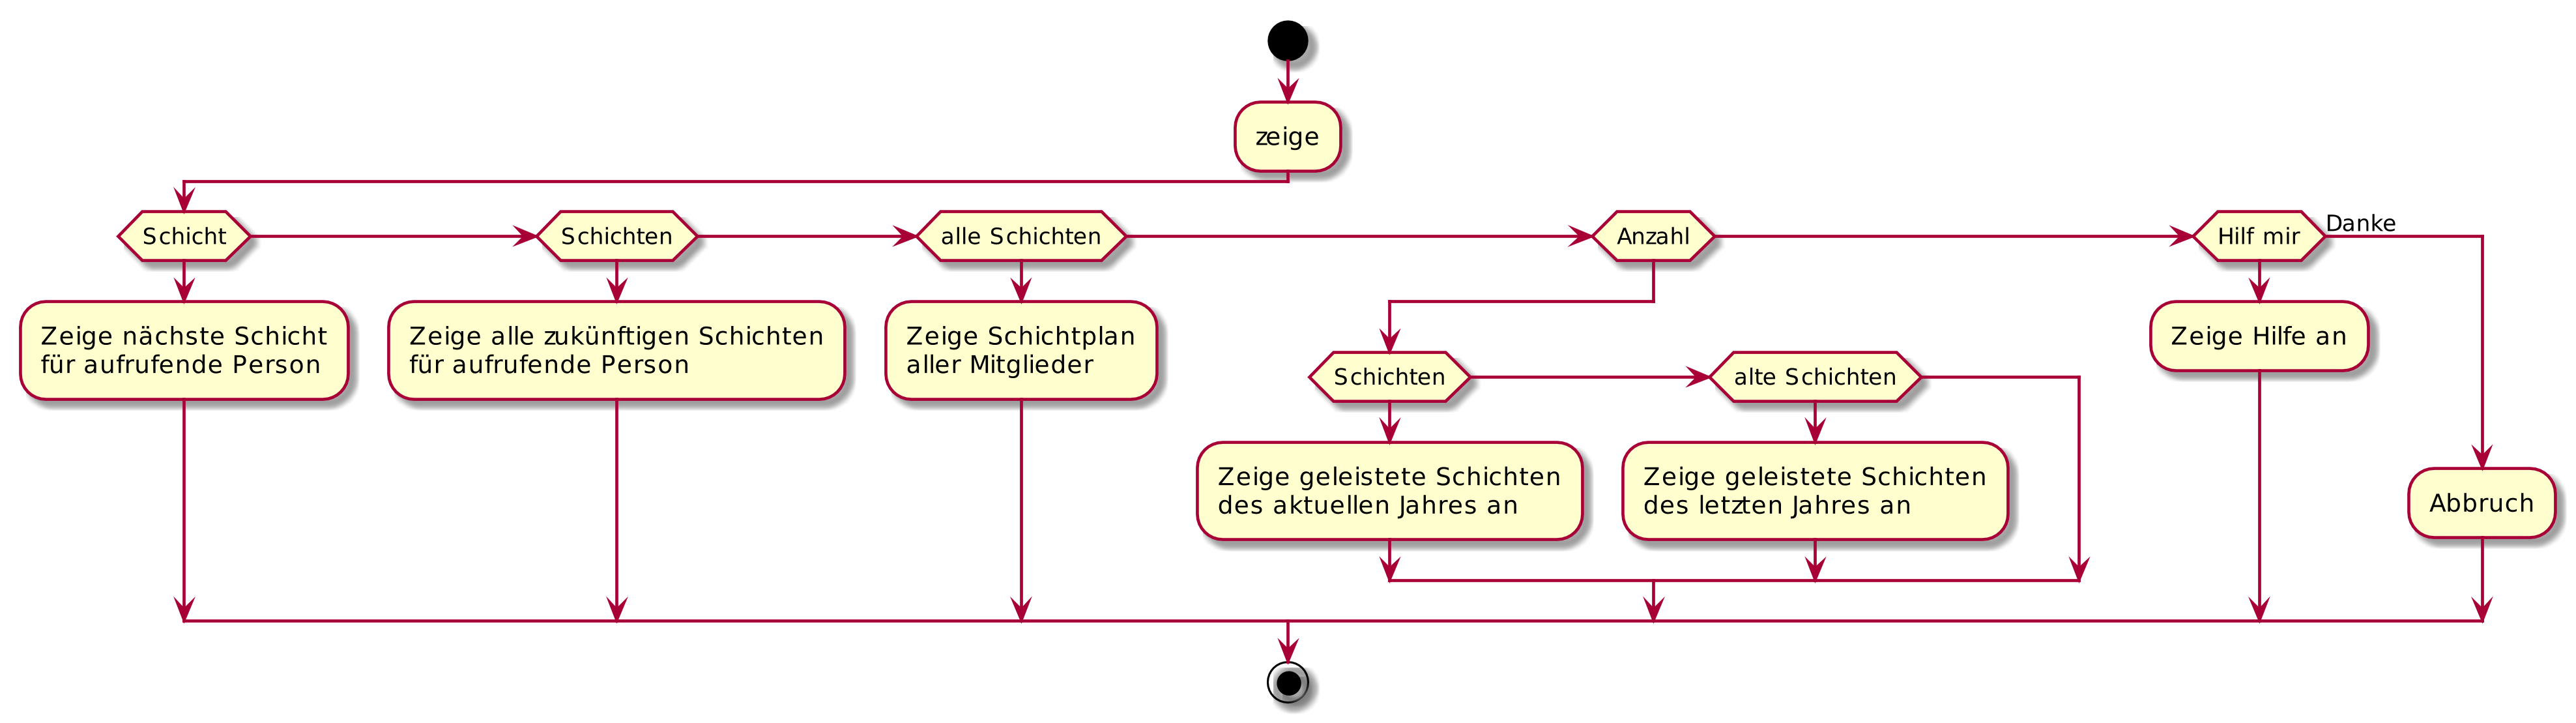
\includegraphics[width=\textwidth]{../docs/uml/activity-zeige.png}
    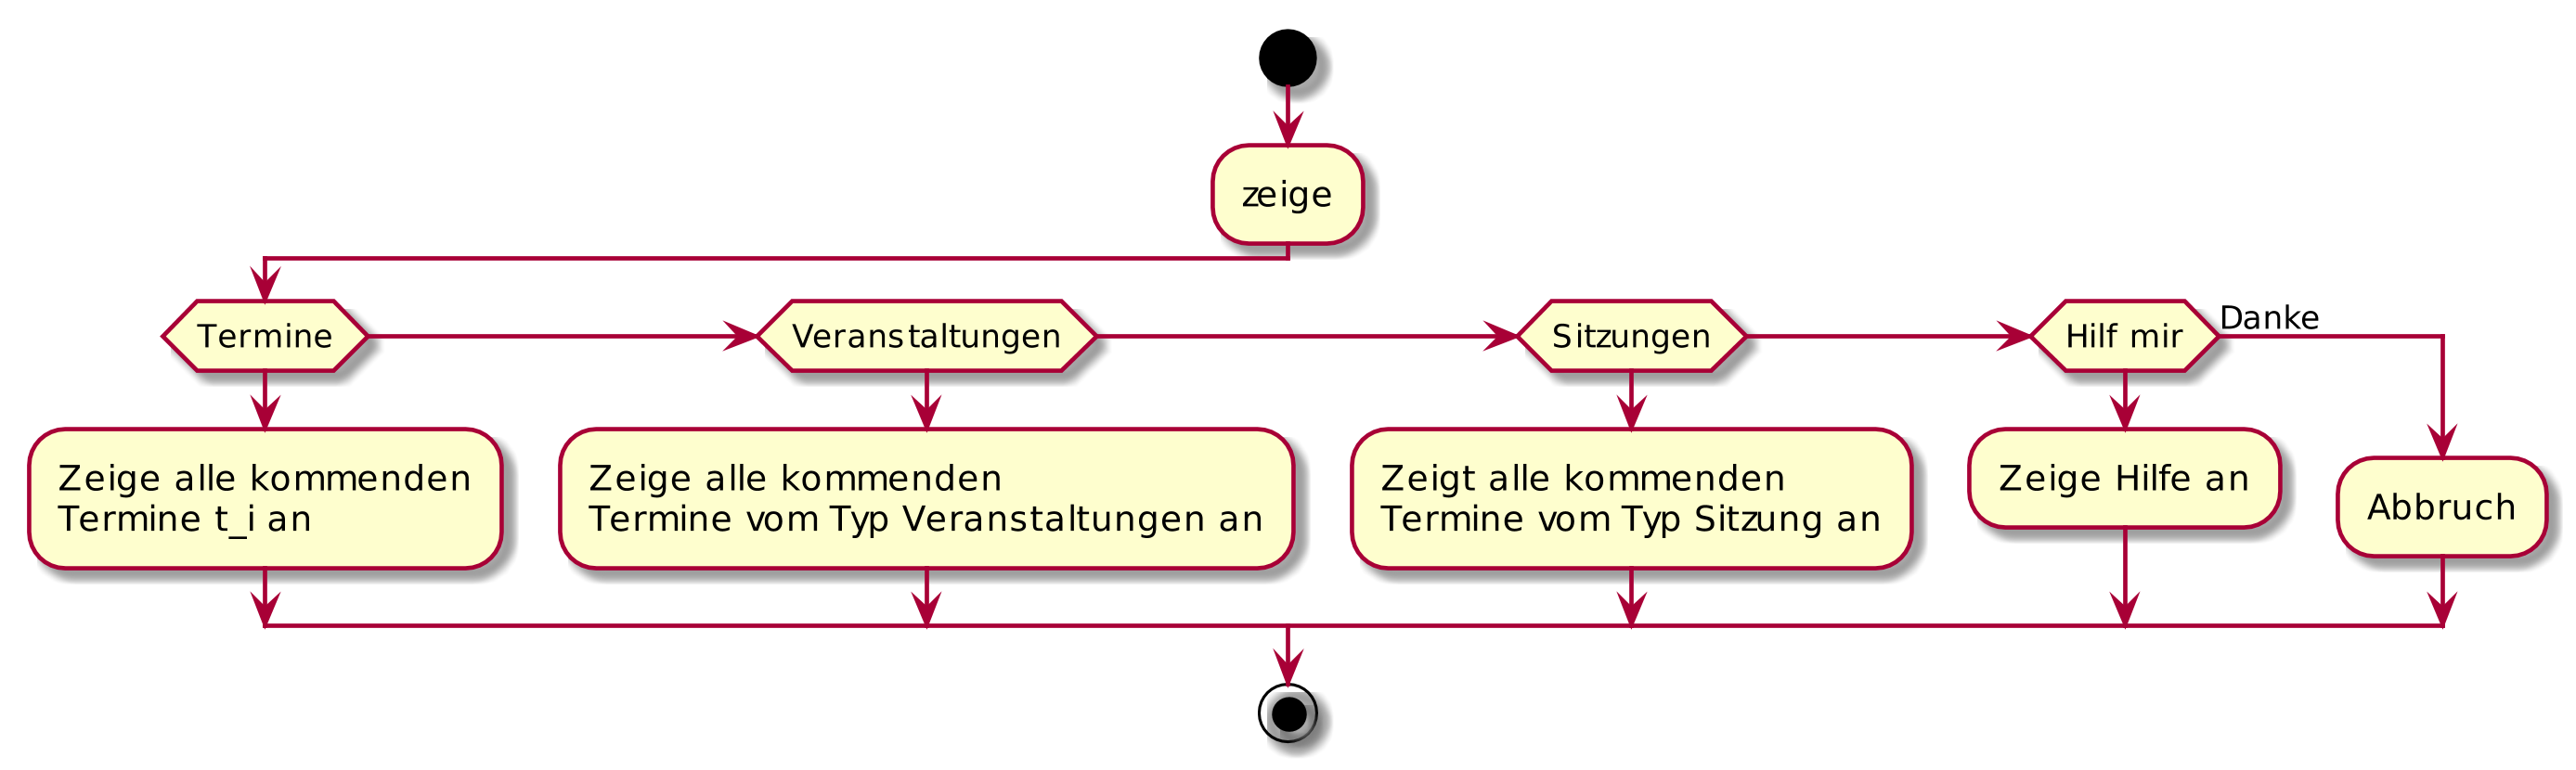
\includegraphics[width=0.9\textwidth]{../docs/uml/activity-zeige2.png}
    \caption{Aktivitätsdiagramme zum Anzeigen von Terminen}
    \label{img:activity-zeige}
\end{figure}

\begin{figure}[htbp]
    \centering
    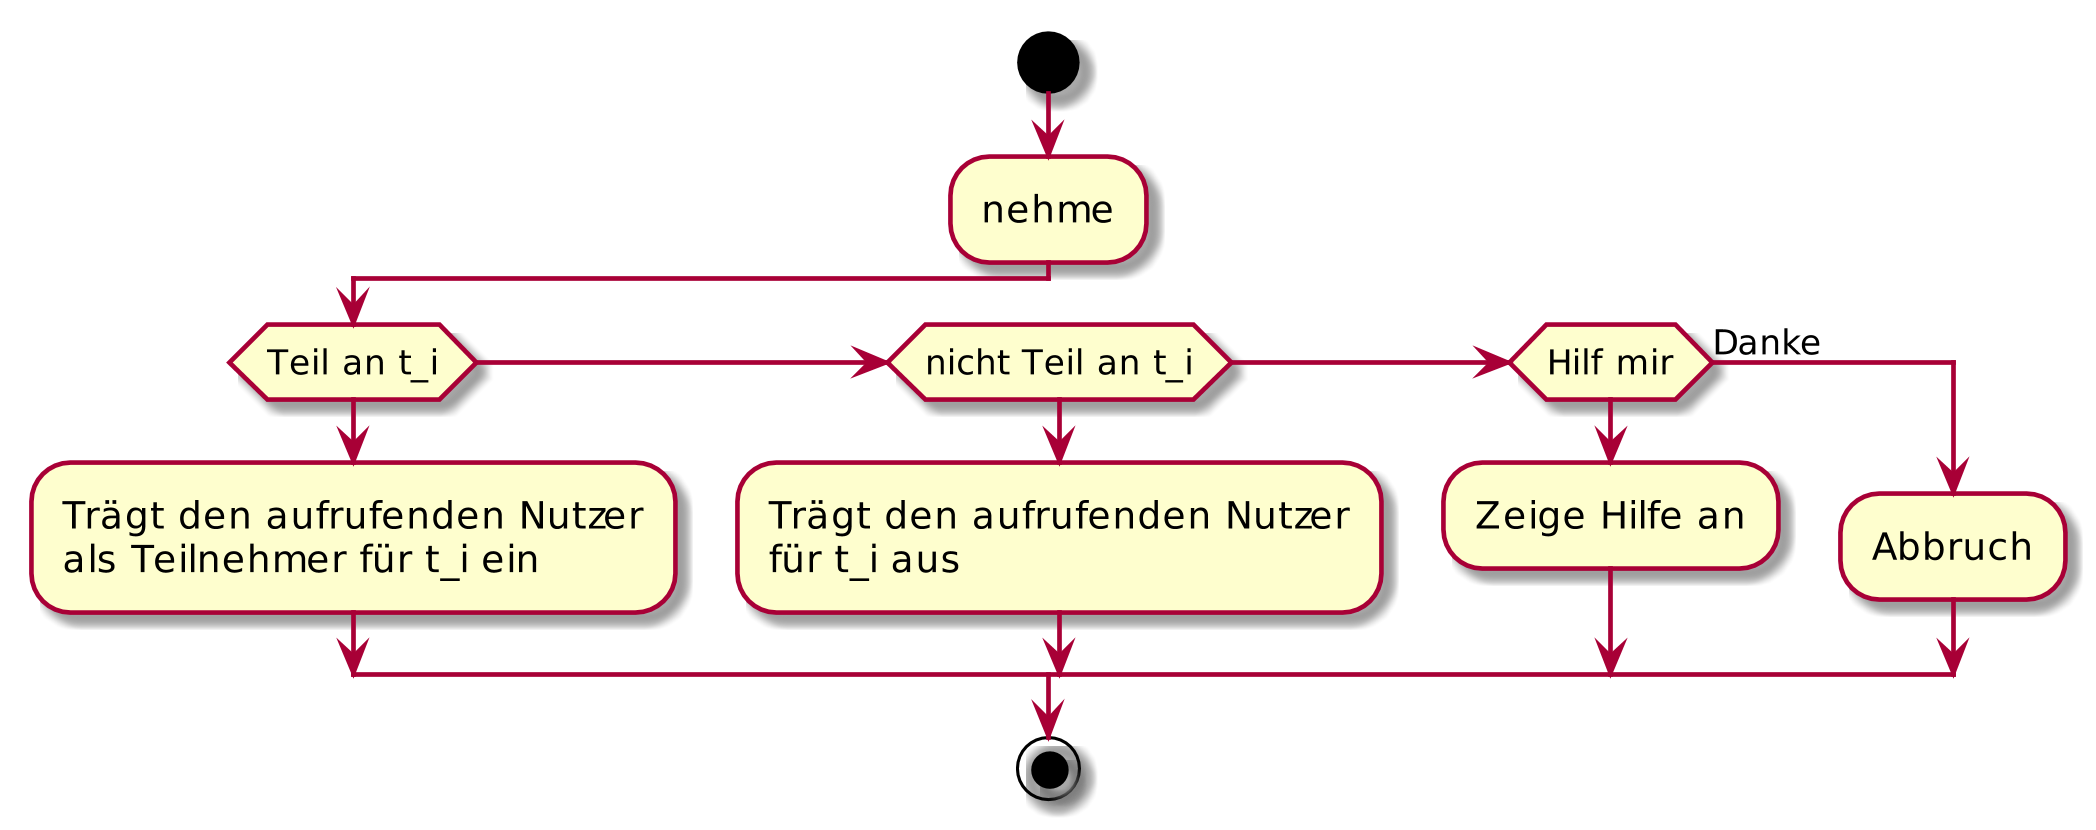
\includegraphics[width=0.7\textwidth]{../docs/uml/activity-teilnahme.png}
    \caption{Aktivitätsdiagramm zur Teilnahme an Terminen}
    \label{img:activity-teilnahme}
\end{figure}


\subsection{Datenbankschema}

Das Datenbankschema soll laut Anforderung unabhängig von einem spezifischen Chatbot nutzbar sein. Falls ein Chatbot ausgetauscht oder andere Interaktionsmethoden hinzugefügt werden, darf die Datenbank entsprechend keine Abhängigkeiten besitzen. Es wird deshalb ein Datenbankschema angelegt, welches nur die Terminverwaltung abbildet und anschließend eine Erweiterung hinzugefügt, welche die notwendigen Schlüssel auf die verwendete Plattform abbildet.

% Hier das DB-Schmea rein und eine Fremdschlüsseltabelle für die Slack-Nutzernamen und bla

\begin{figure}[htbp]
    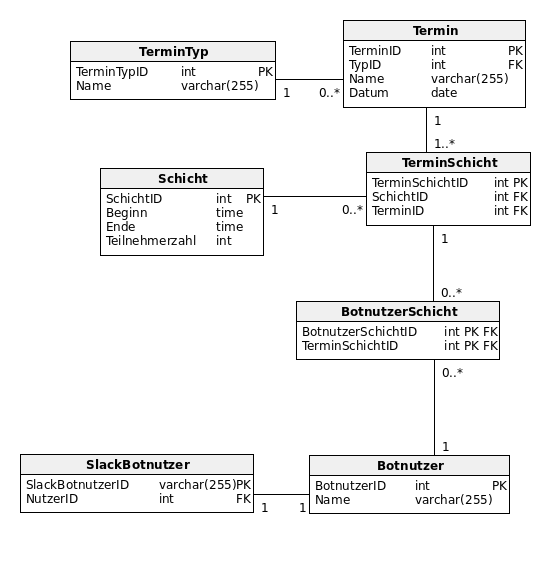
\includegraphics[width=\textwidth]{../docs/uml/Steckerbot-DB.png}
    \caption{Schema für die Termin-DB}
    \label{img:db-schema}
\end{figure}


\subsection{Kommunikationsschnittstellen}

Die kommunikation zwischen der Datenbank und dem Chatbot erfolgt auf dem gleichen Host, weshalb keine besonderen Fälle beachtet werden müssen. Der Kommunikationspfad zwischen dem Chatbot und Slack wird jedoch über ein Hochschulnetzwerk durchgeführt. In diesem sind in das Netzwerk des Clubs nur die Ports 80 und 443 freigegeben. Ausgehend ????????????????? doppeltes NAT aber Webseiten ok

Aus diesem Grund muss der Chatbot sich als Client mit Slack verbinden und darf keine Serveranwendung sein, welche ein Polling implementiert.

% vllt Grafik einfügen?


TODO: ERWEITERN
Slack hat eine option globale UIDs zum bot durchzuleiten. nützlich, wenn mehrere Workspaces genutzt werden - ist das der fall? ferdi fragen.
